\documentclass[11pt, a4paper]{article}
\usepackage{pdfpages}
\usepackage{parallel}
\usepackage[T2A]{fontenc}
%\usepackage{ucs}
\usepackage[utf8]{inputenc}
\usepackage[english,russian]{babel}
\usepackage{hyperref}
\usepackage{rotating}
\usepackage[inner=2cm,top=1.8cm,outer=2cm,bottom=2.3cm,nohead]{geometry}
%\usepackage{listings}
\usepackage{graphicx}
\usepackage{wrapfig}
\usepackage{longtable}
\usepackage{indentfirst}
\usepackage{array}
\usepackage{tikzsymbols}
\usepackage{soul}
\usepackage[ruled,vlined]{algorithm2e}
\usepackage{qrcode}
\counterwithout{figure}{section} 

\usepackage{url}
\makeatletter
\g@addto@macro{\UrlBreaks}{\UrlOrds}
\makeatother

\newcolumntype{P}[1]{>{\raggedright\arraybackslash}p{#1}}
\frenchspacing
%\usepackage{fixltx2e} %text sub- and superscripts
\usepackage{icomma} % коскі ў матэматычным рэжыме
%\PreloadUnicodePage{4}

\newcommand{\longpage}{\enlargethispage{\baselineskip}}
\newcommand{\shortpage}{\enlargethispage{-\baselineskip}}

\def\switchlang#1{\expandafter\csname switchlang#1\endcsname}
\def\switchlangbe{
\let\saverefname=\refname%
\def\refname{Літаратура}%
\def\figurename{Іл.}%
}
\def\switchlangru{
\let\saverefname=\refname%
\let\savefigurename=\figurename%
\def\refname{Литература}%
\def\figurename{Рис.}%
}
\def\switchlangen{
\let\saverefname=\refname%
\def\refname{References}%
\def\figurename{Fig.}%
}

\hyphenation{admi-ni-stra-tive}
\hyphenation{ex-pe-ri-ence}
\hyphenation{fle-xi-bi-li-ty}
\hyphenation{Py-thon}
\hyphenation{ma-the-ma-ti-cal}
\hyphenation{re-ported}
\hyphenation{imp-le-menta-tions}
\hyphenation{pro-vides}
\hyphenation{en-gi-neering}
\hyphenation{com-pa-ti-bi-li-ty}
\hyphenation{im-pos-sible}
\hyphenation{desk-top}
\hyphenation{elec-tro-nic}
\hyphenation{com-pa-ny}
\hyphenation{de-ve-lop-ment}
\hyphenation{de-ve-loping}
\hyphenation{de-ve-lop}
\hyphenation{da-ta-ba-se}
\hyphenation{plat-forms}
\hyphenation{or-ga-ni-za-tion}
\hyphenation{pro-gramming}
\hyphenation{in-stru-ments}
\hyphenation{Li-nux}
\hyphenation{sour-ce}
\hyphenation{en-vi-ron-ment}
\hyphenation{Te-le-pathy}
\hyphenation{Li-nux-ov-ka}
\hyphenation{Open-BSD}
\hyphenation{Free-BSD}
\hyphenation{men-ti-on-ed}
\hyphenation{app-li-ca-tion}

\def\progref!#1!{\texttt{#1}}
\renewcommand{\arraystretch}{2} %Іначай формулы ў матрыцы зліпаюцца з лініямі
\usepackage{array}

\def\interview #1 (#2), #3, #4, #5\par{

\section[#1, #3, #4]{#1 -- #3, #4}
\def\qname{LVEE}
\def\aname{#1}
\def\q ##1\par{{\noindent \bf \qname: ##1 }\par}
\def\a{{\noindent \bf \aname: } \def\qname{L}\def\aname{#2}}
}

\def\interview* #1 (#2), #3, #4, #5\par{

\section*{#1\\{\small\rm #3, #4. #5}}
\ifx\ParallelWhichBox\undefined%
    \addcontentsline{toc}{section}{#1, #3, #4}%
\else%
\ifnum\ParallelWhichBox=0%
    \addcontentsline{toc}{section}{#1, #3, #4}%
\fi\fi%

\def\qname{LVEE}
\def\aname{#1}
\def\q ##1\par{{\noindent \bf \qname: ##1 }\par}
\def\a{{\noindent \bf \aname: } \def\qname{L}\def\aname{#2}}
}

\newcommand{\interviewfooter}[1]{
\vskip 1em
\noindent \textit{#1}
}

\AtEndDocument{\vfill\centering \qrcode{https://github.com/fiowro/mouses/blob/main/\jobname.pdf}}

\switchlang{ru}
\begin{document}

\title{1987 "--- Трекбол/мышь Sharp KI-OM0002CE01}
\date{}
\maketitle
\selectlanguage{russian}

В 1986 году компания Sharp анонсировала для японского рынка выпуск 16-битного персонального компьютера  X68000 на базе процессора Motorola 68000. Компьютер поступили в продажу в марте 1987. Он позиционировался как персональная рабочая станция, и сразу привлек внимение из-за богатых возможностей для работы с графикой и воспроизведения аудио (не уступавших лучшим игровым консолям конца 80х годов), дополненных необычным дизайном системного блока в сдвоенном вертикальном корпусе \cite{museum}. В комплекте с этим компьютером поставлялась необычная мышь-перевертыш (рис. \ref{fig:SharpConvertibleMouse}), которая могла дополнительно работать как в режиме трекбола. Поскольку устройство не предназначалось для отдельной продажи, оно получило труднозапоминающийся модельный номер KI-OM0002CE01 (при выпуске последующих поколений компьютеров X68000 номер модели мыши увеличивался на единицу, однако сама она не претерпевала заметных изменений).

\begin{figure}[h]
    \centering
    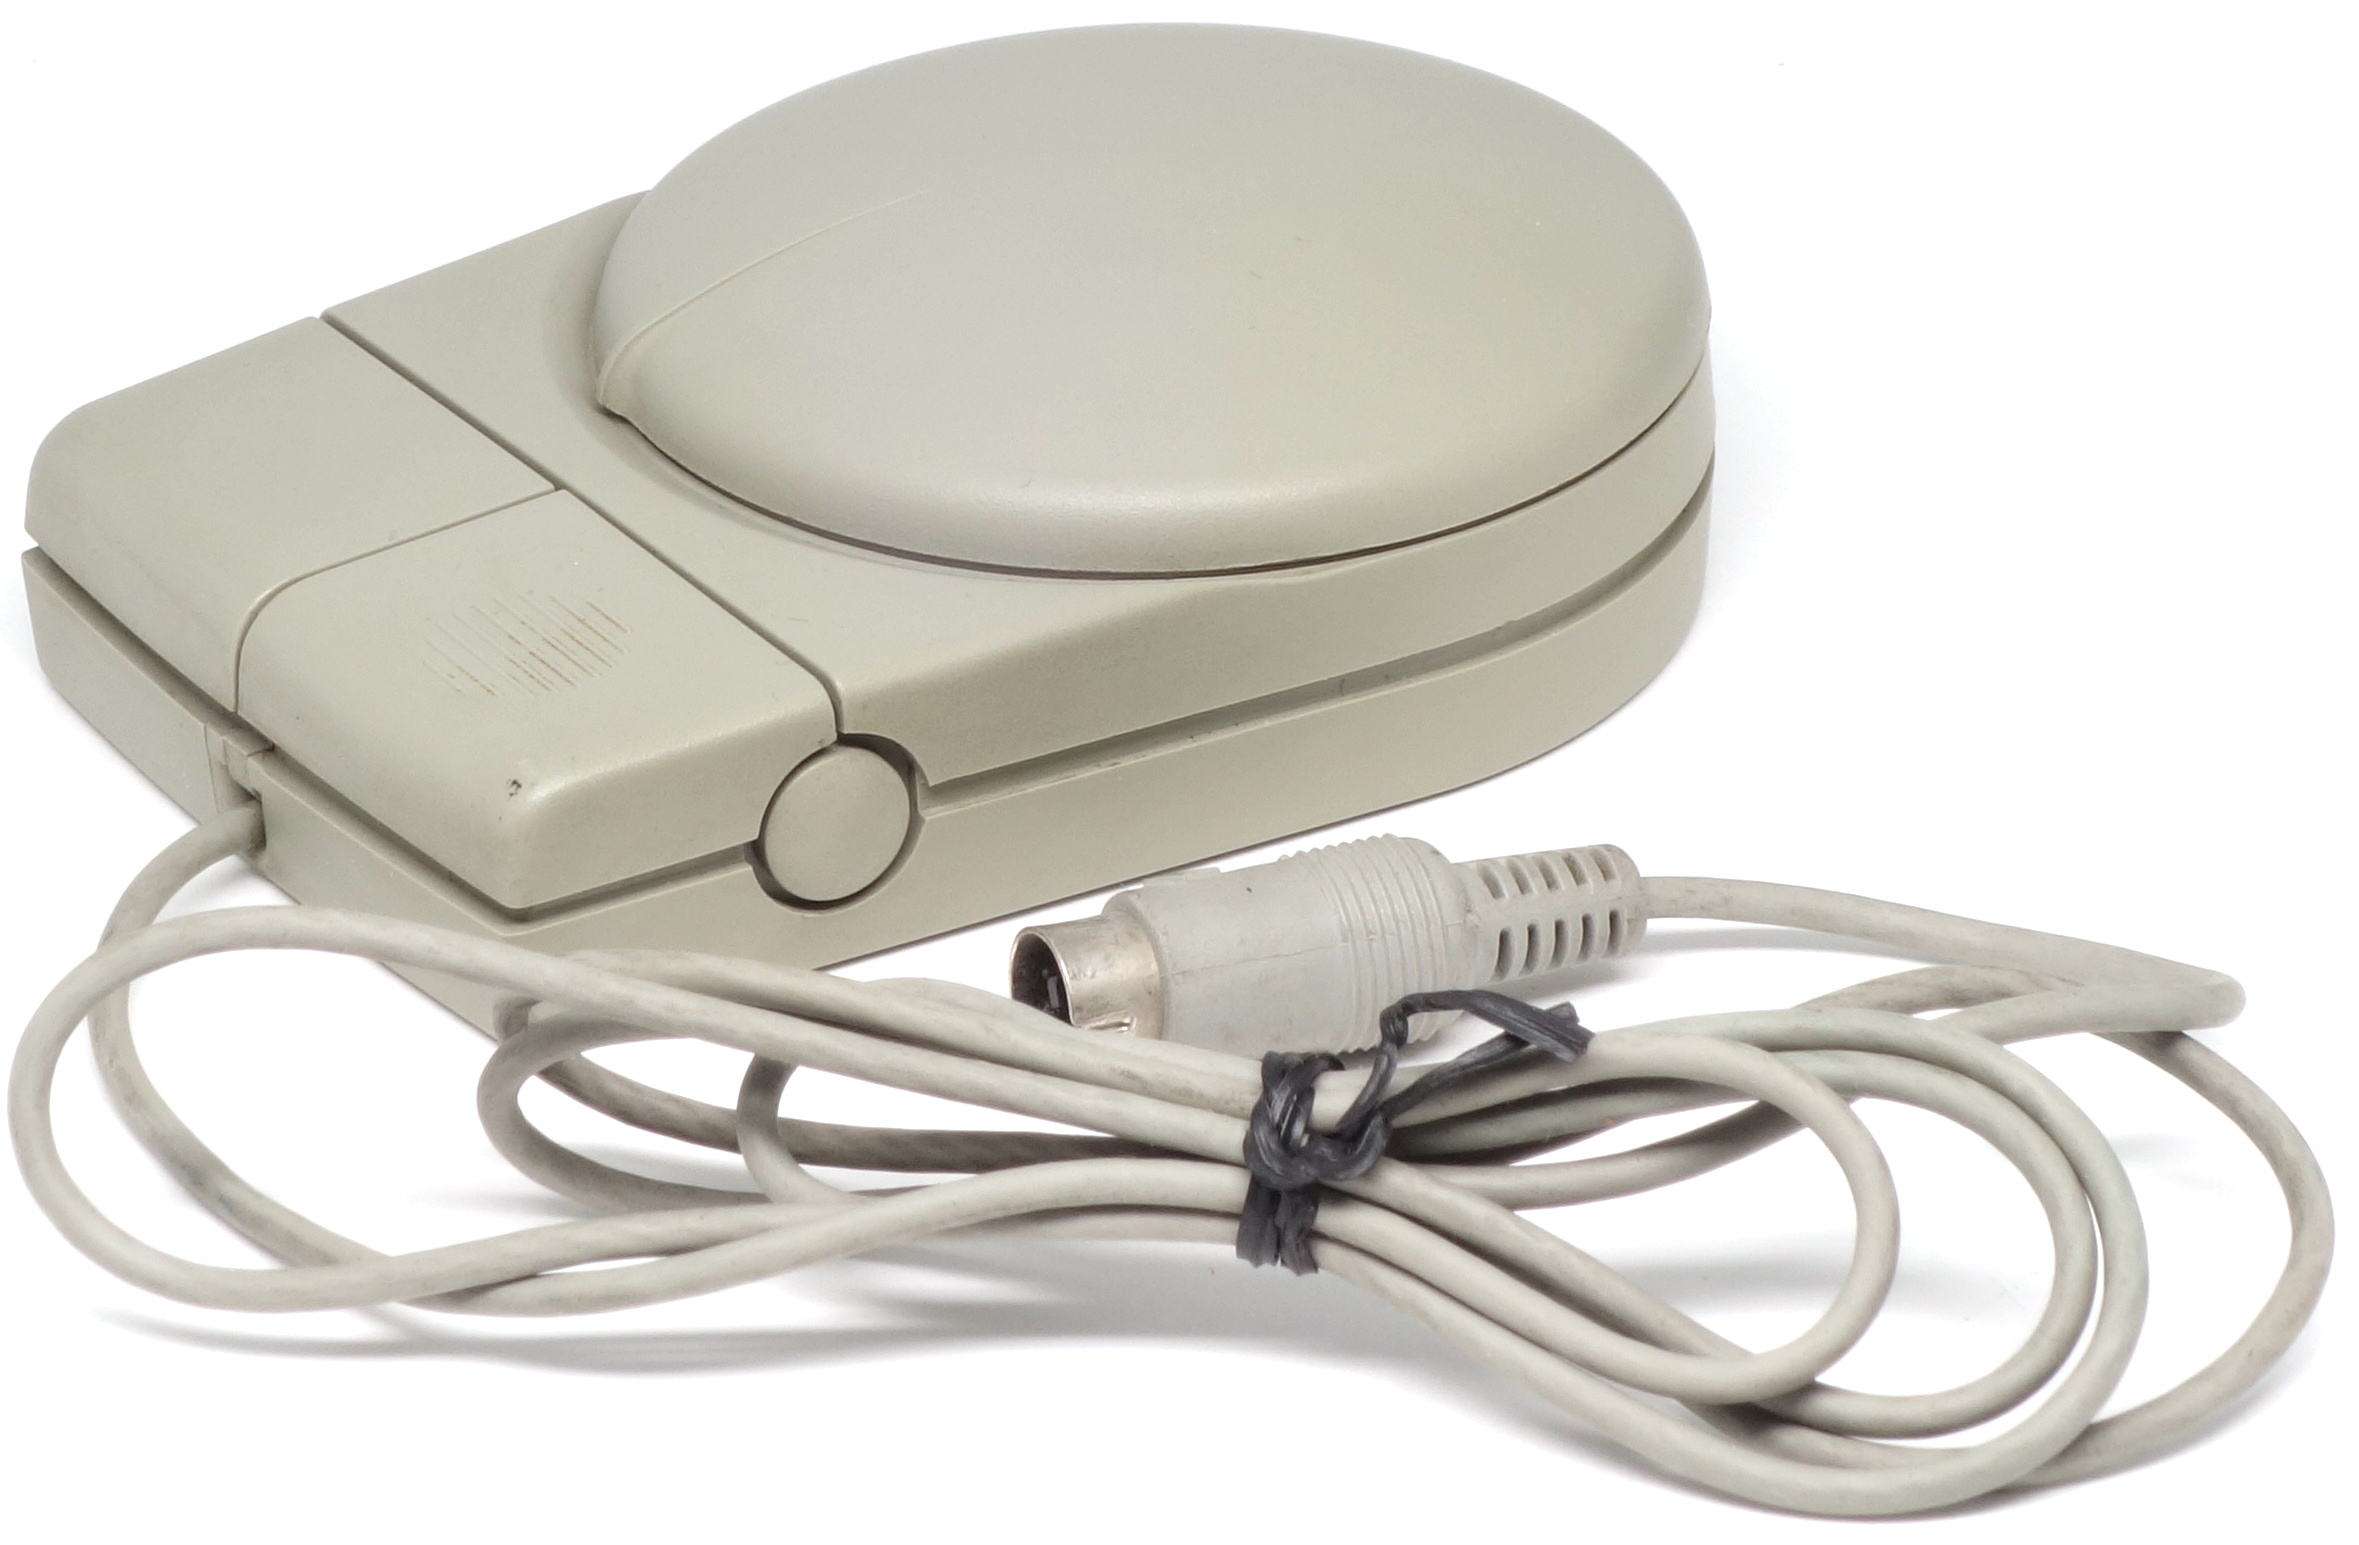
\includegraphics[scale=0.65]{1987_sharp_convertible/picmouse_60}
    \caption{Изображение Sharp KI-OM0002CE01 в режиме мыши}
    \label{fig:SharpConvertibleMouse}
\end{figure}

\begin{figure}[h]
    \centering
    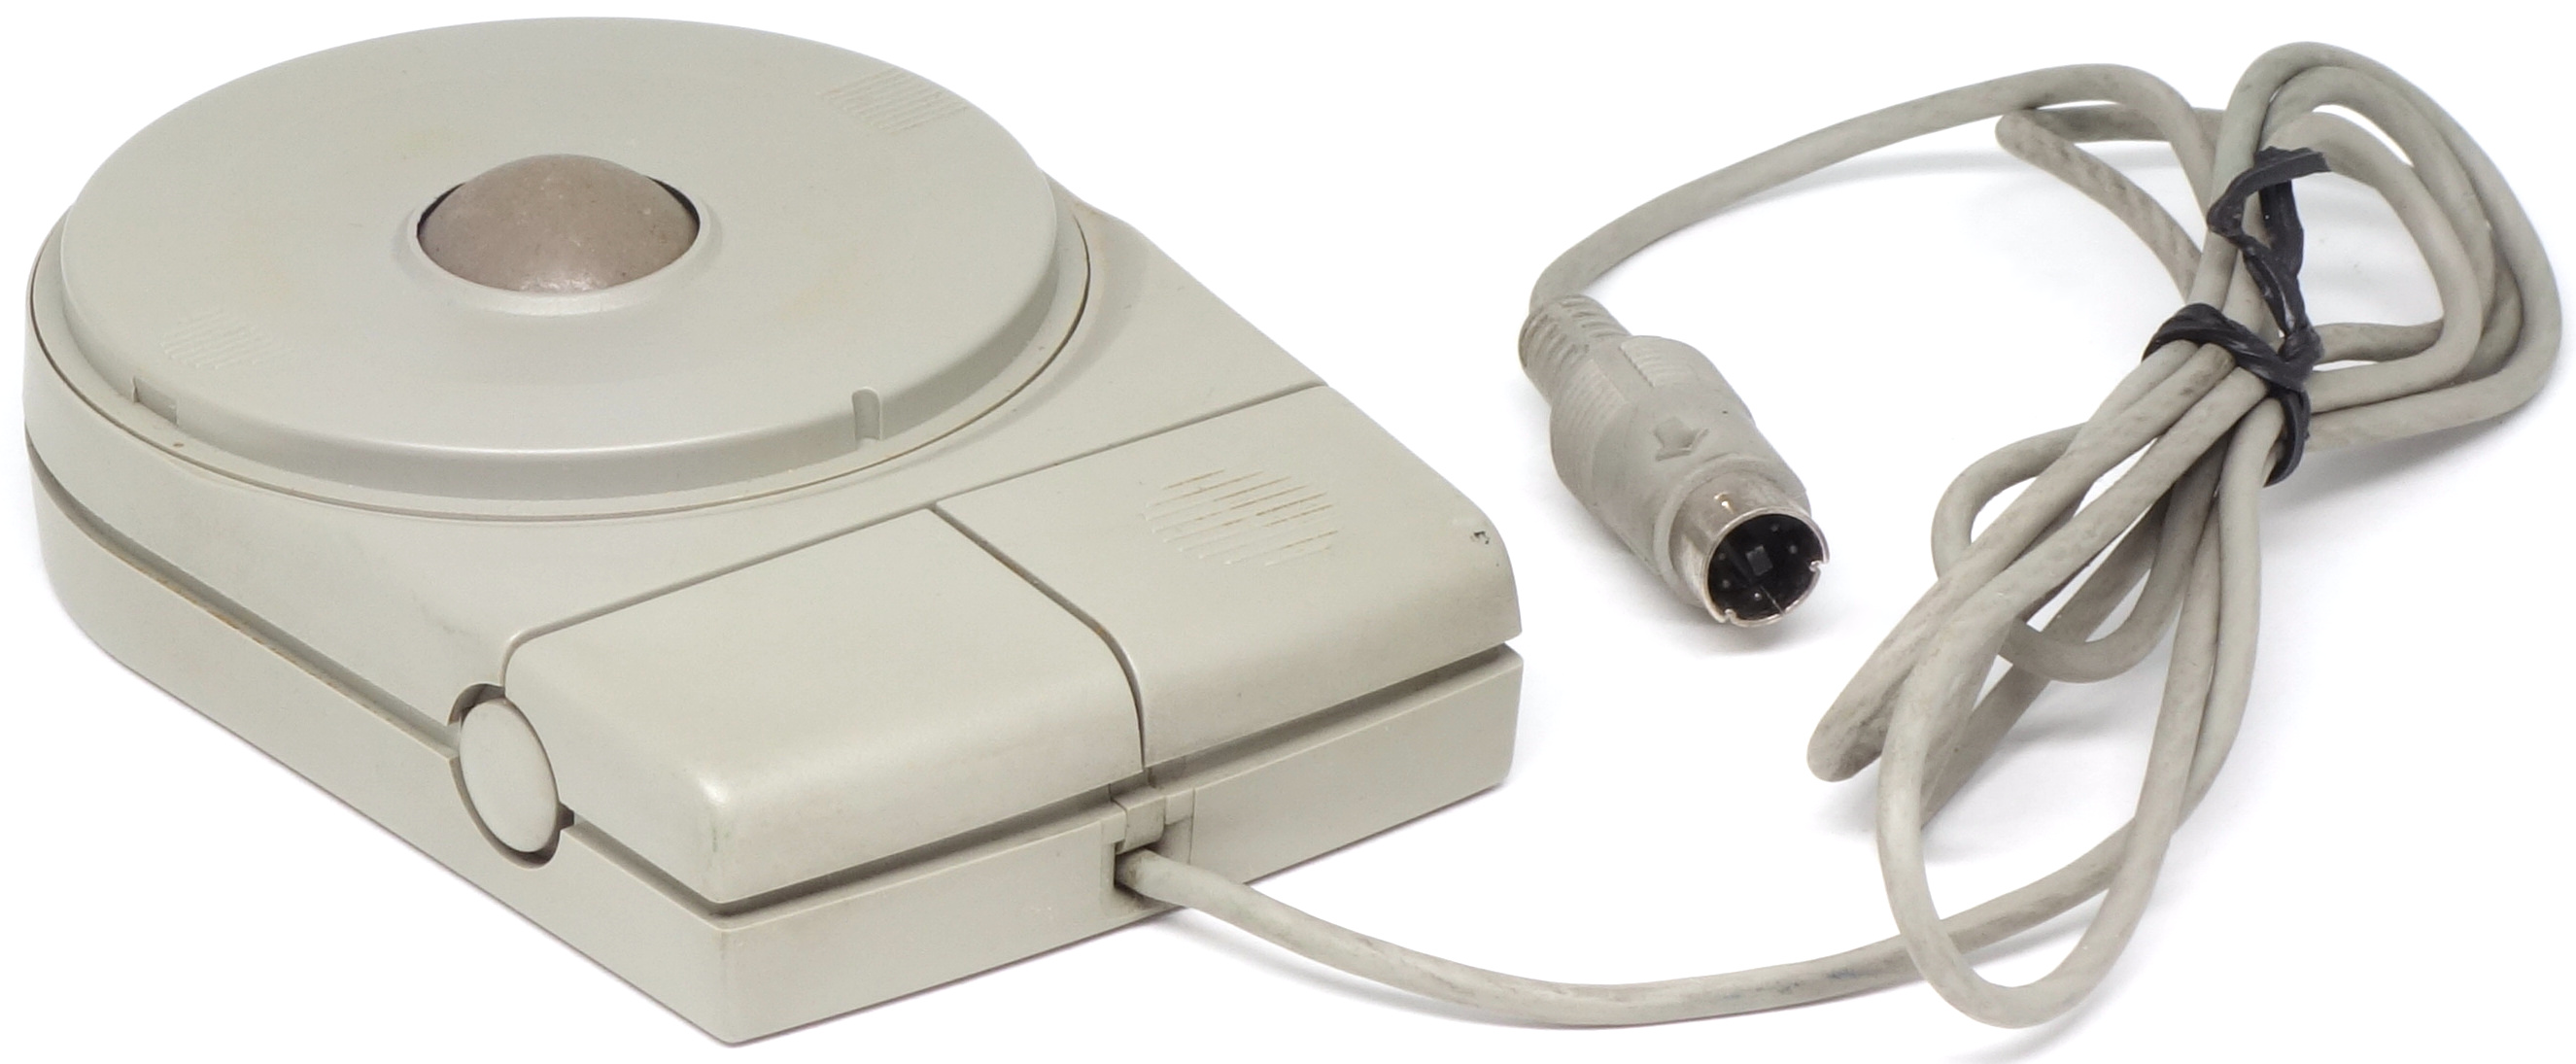
\includegraphics[scale=0.65]{1987_sharp_convertible/picball_60}
    \caption{Изображение Sharp KI-OM0002CE01 в режиме трекбола}
    \label{fig:SharpConvertibleTrackball}
\end{figure}

В дизайне мыши чувствуется приверженность к строгой геометрии; nакже можно заметить сходство общей формы корпуса с мышью HP 46060A, разработанной в 1984 году Logitech для компьютеров компании Hewlett Packard. Корпус мыши достаточно плоский, с двумя кнопками большого размера и дополнительными маленькими боковыми кнопками по бокам, дублирующими функции основных кнопок \cite{JapaneseVintage}. Две трети корпуса занимает съемная круглая крышка (рис. \ref{fig:SharpConvertibleMouse}), служащая опорой для ладони и одновременно закрывающая шар. Поворот крышки на 90\,$^\circ$ позволяет подцепить ее за выступ и снять, чтобы использовать устройство в режиме трекбола (рис. \ref{fig:SharpConvertibleTrackball}). Сама крышка крепится к корпусу на защелках и не является поворотной; на самом деле вращается центральная часть корпуса, содержащая в себе механический узел устройства и часть электроники.

\begin{figure}[h]
    \centering
    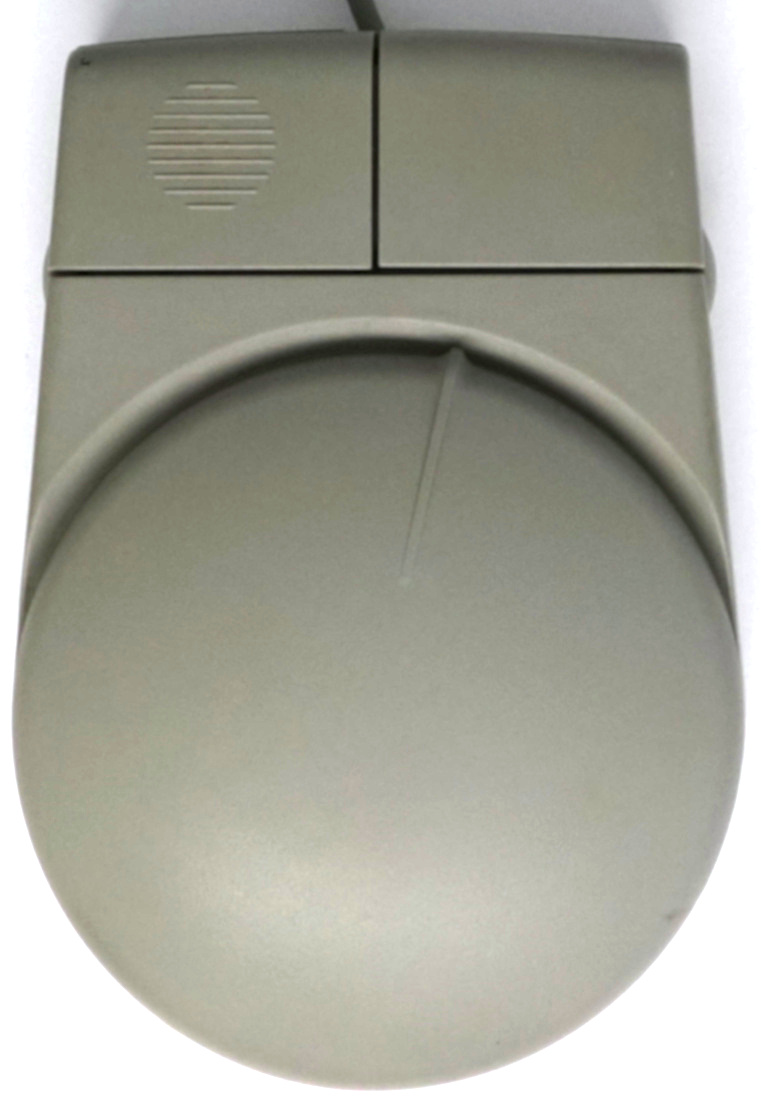
\includegraphics[scale=0.6]{1987_sharp_convertible/top_30.jpg}
    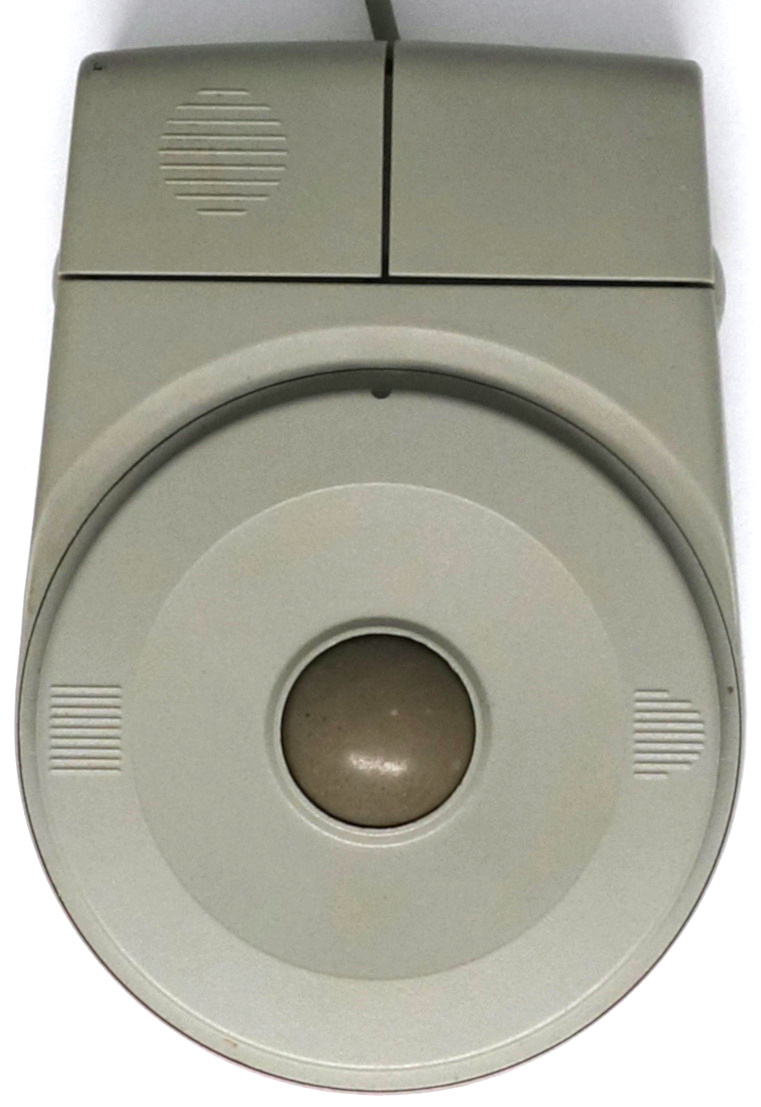
\includegraphics[scale=0.6]{1987_sharp_convertible/topball_30.jpg}
    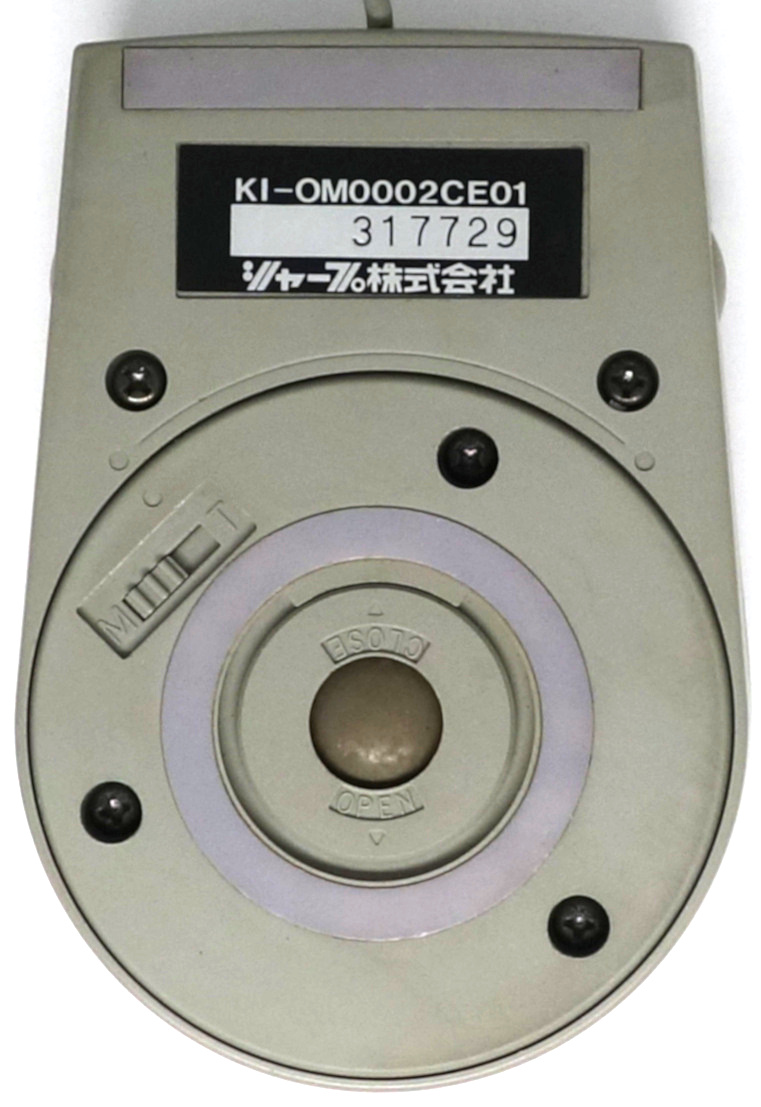
\includegraphics[scale=0.6]{1987_sharp_convertible/bottom_30.jpg}
    \caption{Изображение Sharp KI-OM0002CE01: вид мыши сверху, вид трекбола сверху, вид снизу}
    \label{fig:SharpConvertibleTopAndBottom}
\end{figure}

Для переключения в режим трекбола помимо снятия крышки необходимо также перевернуть мышь, чтобы шар под действием собственного веса сместился к верхней части корпуса, а затем зафиксировать такое положение шара, переведя переключатель в нижней части мыши из положения <<M>> в <<T>> (рис. \ref{fig:SharpConvertibleTopAndBottom}). Помимо переключателя на нижней стороне корпуса можно заметить низкофрикционные накладки формы, стандартной для мышей, выпускавшихся фирмой Alps по контракту  для других компаний, а также съемное кольцо, позволяющее извлечь шар для чистки.

\begin{figure}[h]
    \centering
    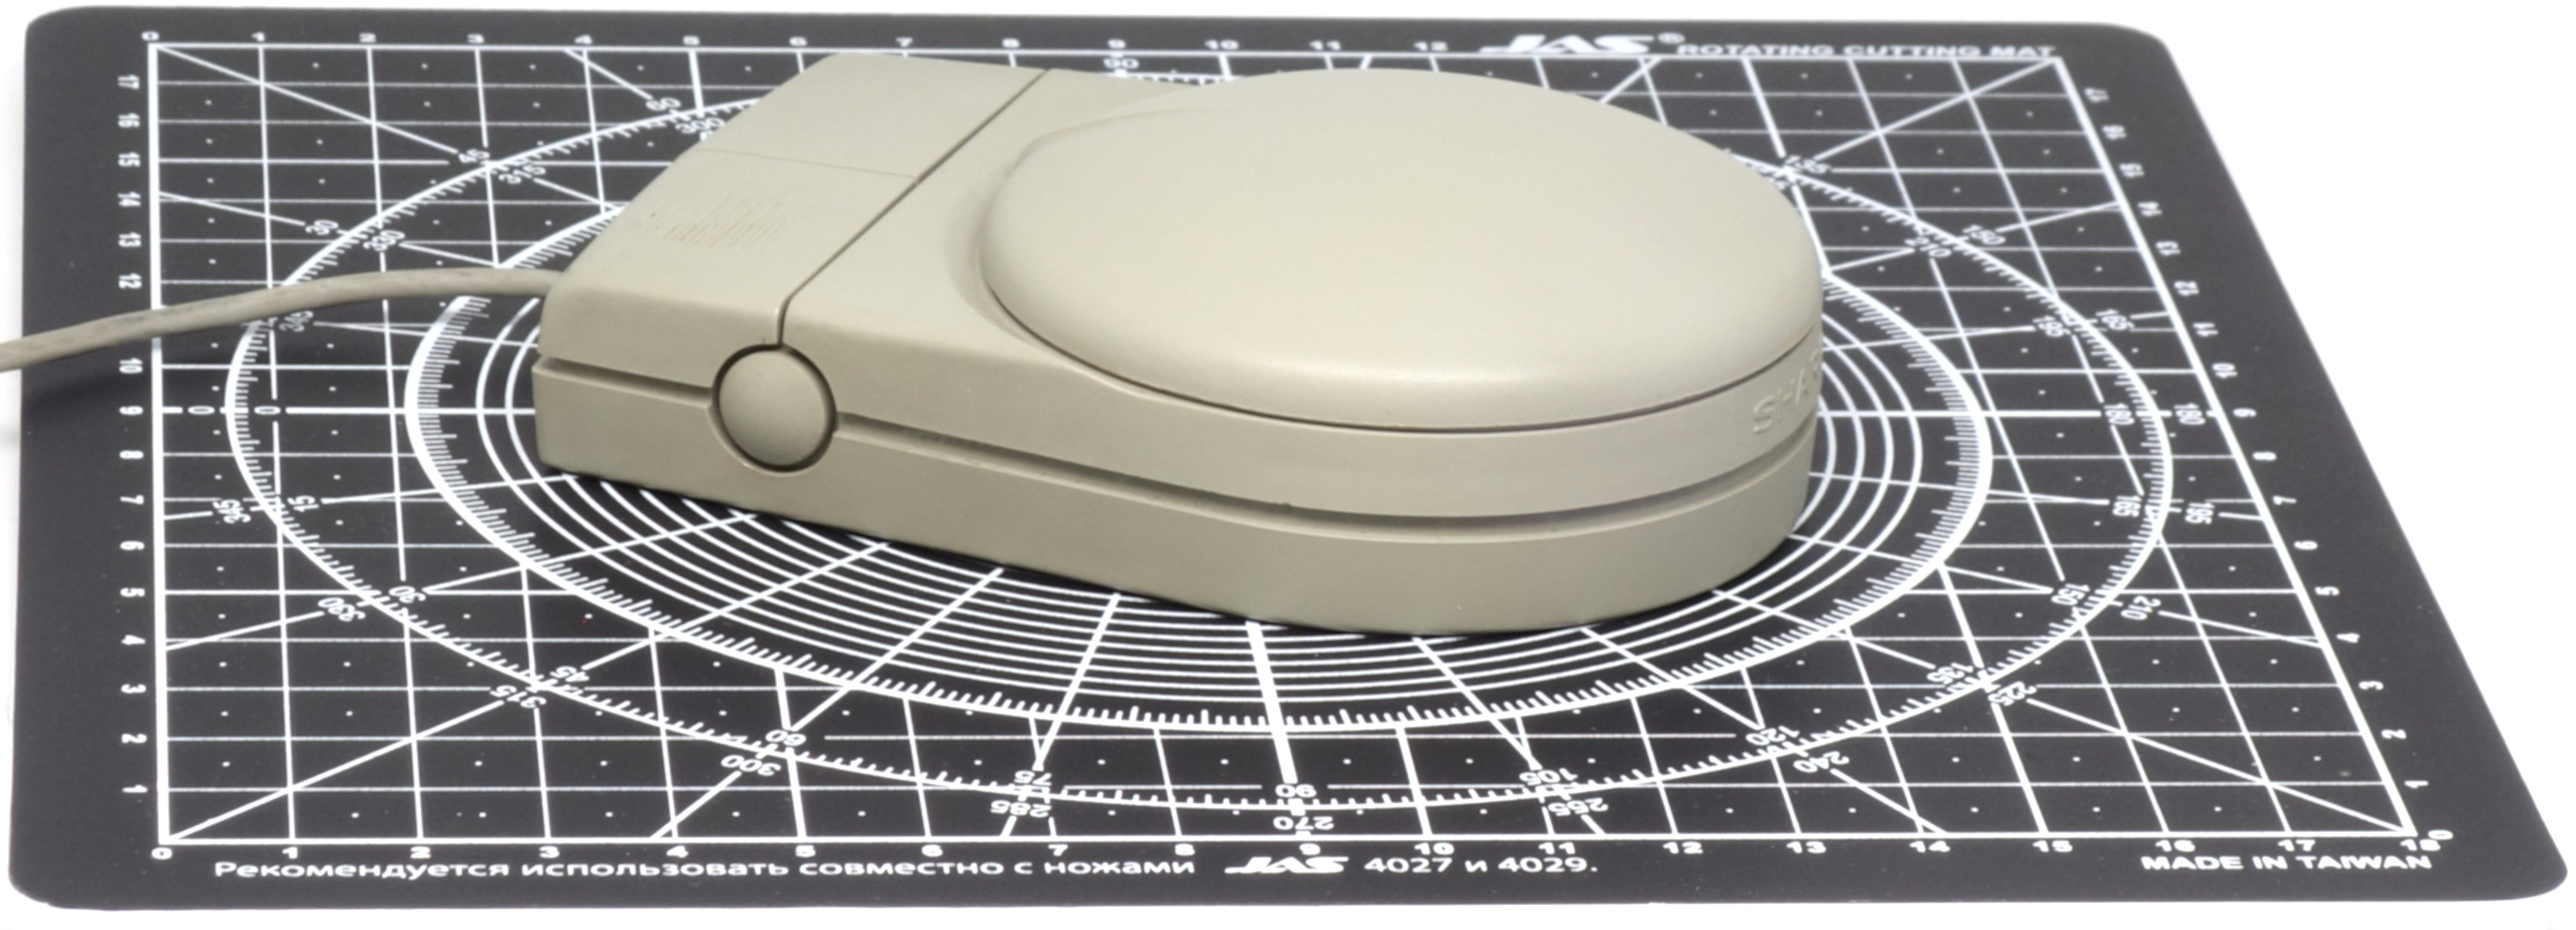
\includegraphics[scale=0.5]{1987_sharp_convertible/size_30.jpg}
    \caption{Изображение KI-OM0002CE01 на размерном коврике с шагом сетки 1~см}
    \label{fig:SharpConvertibleSize}
\end{figure}

Дополнительные элементы и поворотный механизм внутри корпуса не повлияли на размер мыши, типичный для мышей на основе типовых конструкций Alps и для второй половины 80х годов в целом (рис. \ref{fig:SharpConvertibleSize}).

С точки зрения анатомического строения кисти, устройство имеет эргономичную  форму и крупные клавиши, которые удобно нажимать пальцами (рис. \ref{fig:SharpConvertibleHand}). Будучи <<вписанными>> в корпус, как у мышей более позднего периода, кнопки на верхней стороне корпуса имеют более долгий ход, чем-то схожий с ходом клавиш клавиатуры, что очевидно делает пользование мышью чуть менее удобным. Круглая площадка с рельефом на главной кнопке мыши указывает рекомендованное положение для подушечки пальца \cite{JapaneseClickSense}. Аналогичный рельеф нанесен на два участка поворотной части корпуса под крышкой, что призвано облегчить вращение поворотного блока при снятой крышке (рис. \ref{fig:SharpConvertibleTopAndBottom}).

Само наличие поворотного блока позволяет работать в режиме трекбола двумя способами: классическим, когда кнопки расположены за шаром (рис. \ref{fig:SharpConvertibleBallHand}), и когда корпус повернут на 90\,$^\circ$. В этом случае кнопки находятся сбоку, что очевидно предполагает использование устройства двумя руками в режиме геймпада (рис. \ref{fig:SharpConvertiblePadHand}).

\begin{figure}[h]
    \centering
    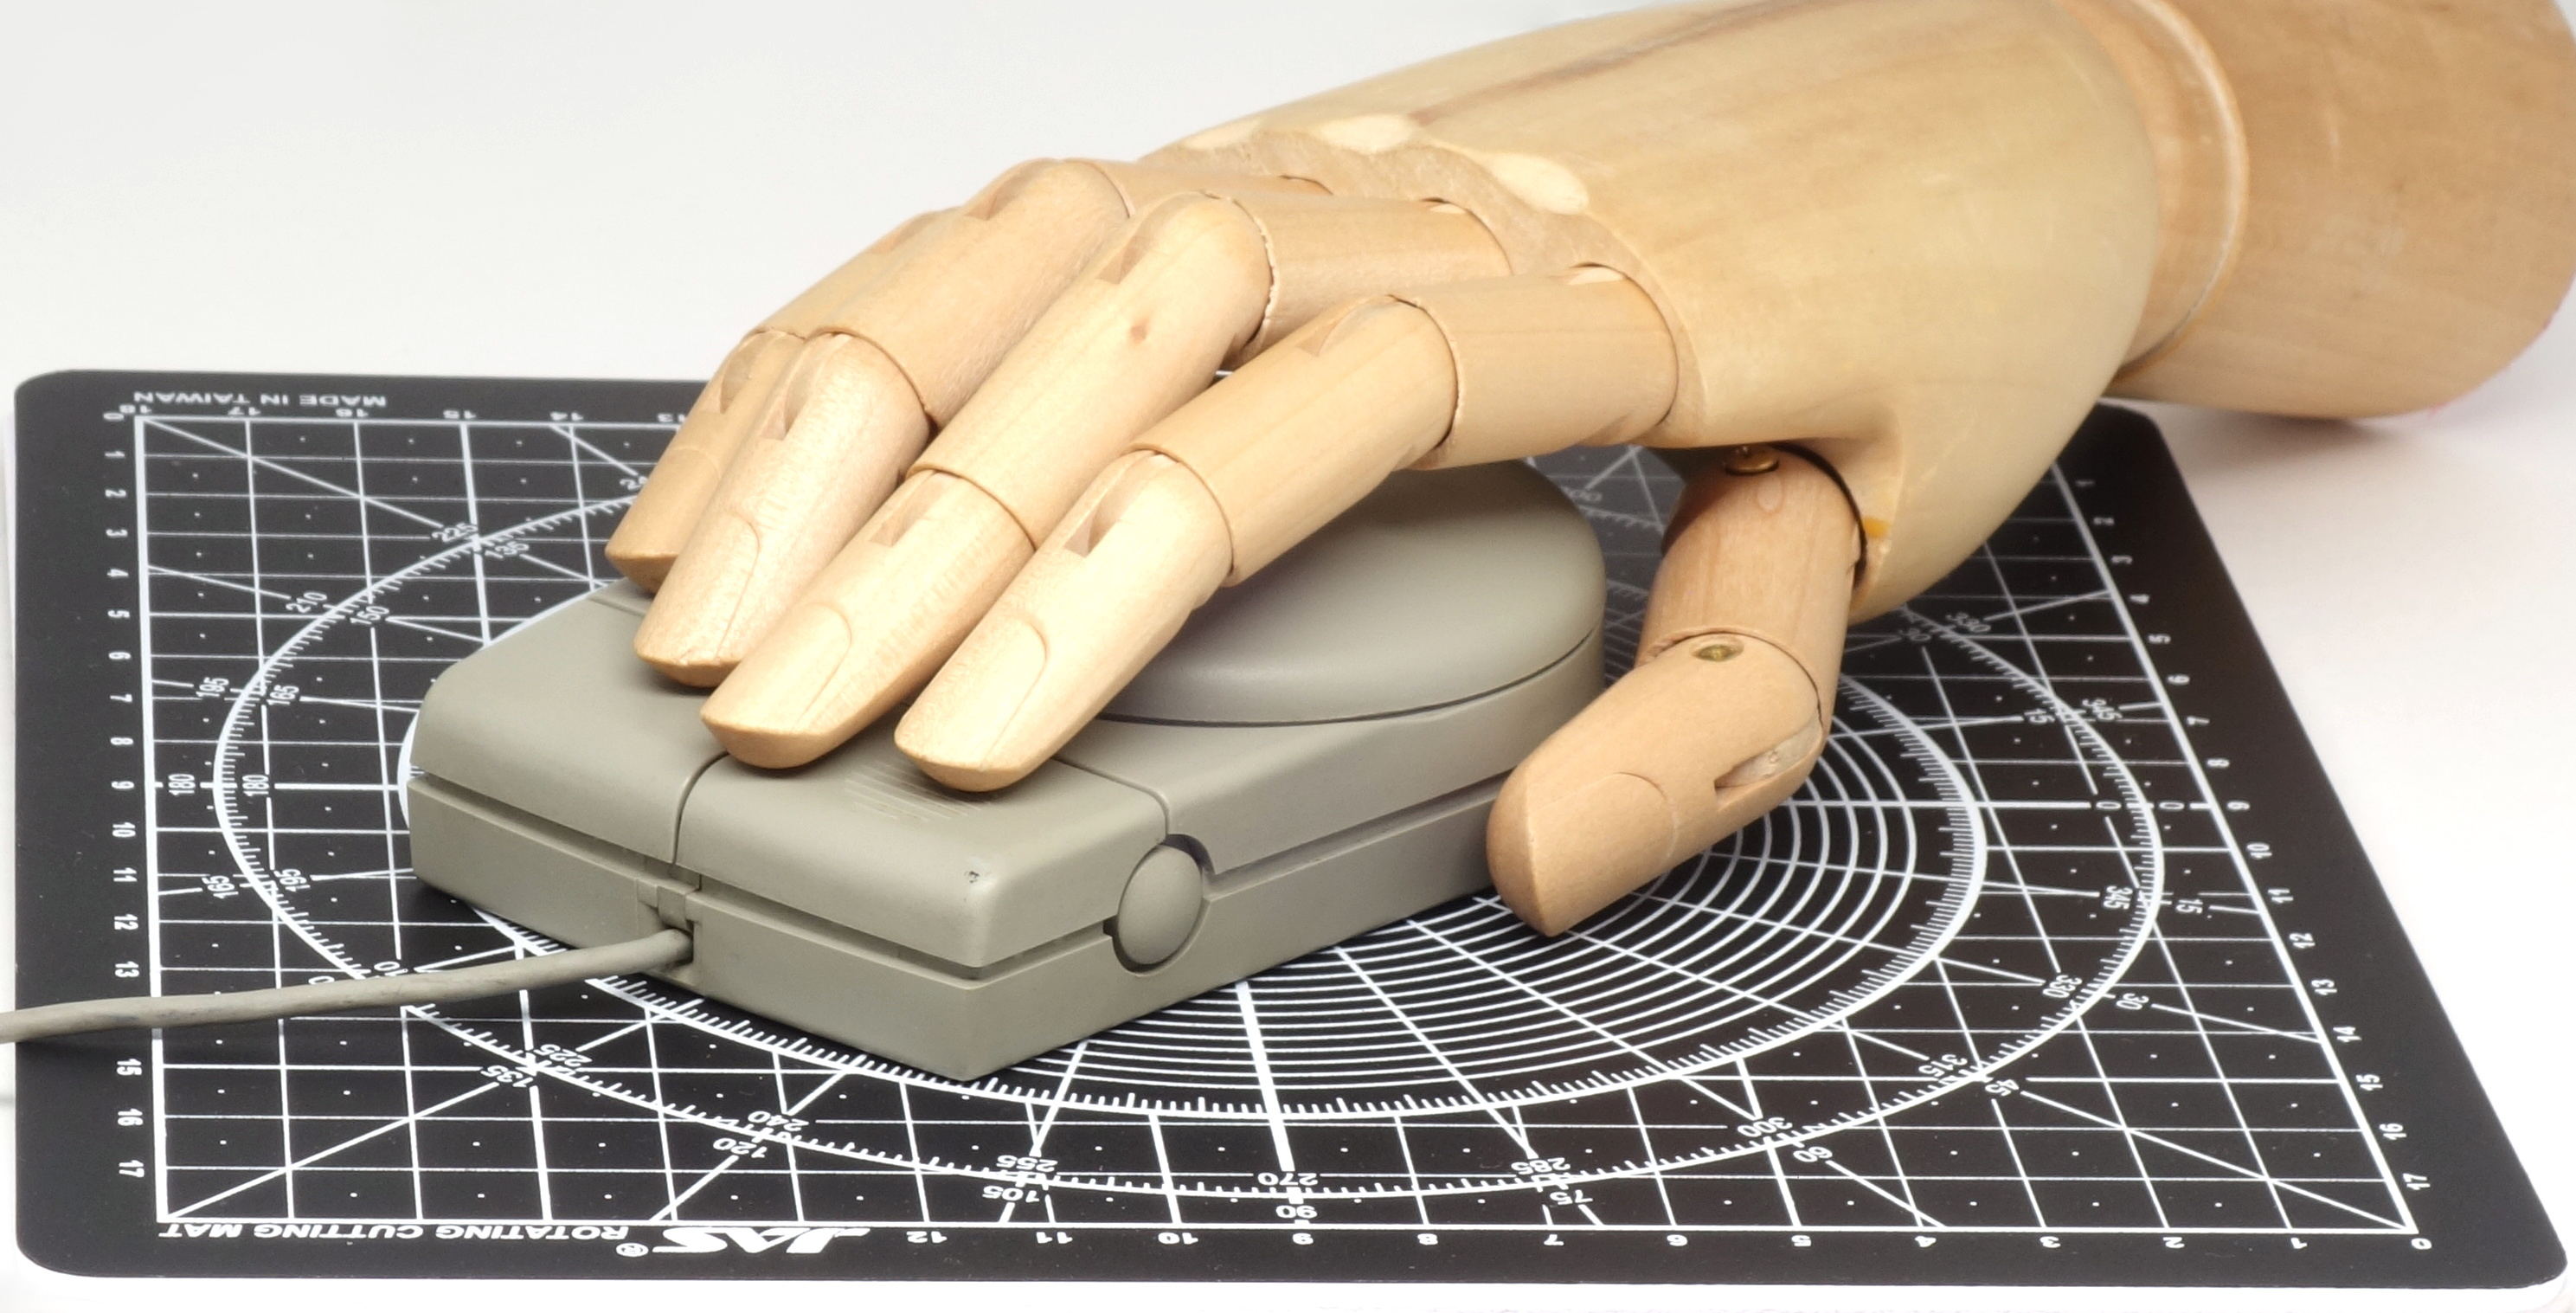
\includegraphics[scale=0.44]{1987_sharp_convertible/handmouse_15.jpg}
    \caption{Sharp KI-OM0002CE01 в режиме мыши с моделью руки человека}
    \label{fig:SharpConvertibleHand}
\end{figure}

\begin{figure}[h]
    \centering
    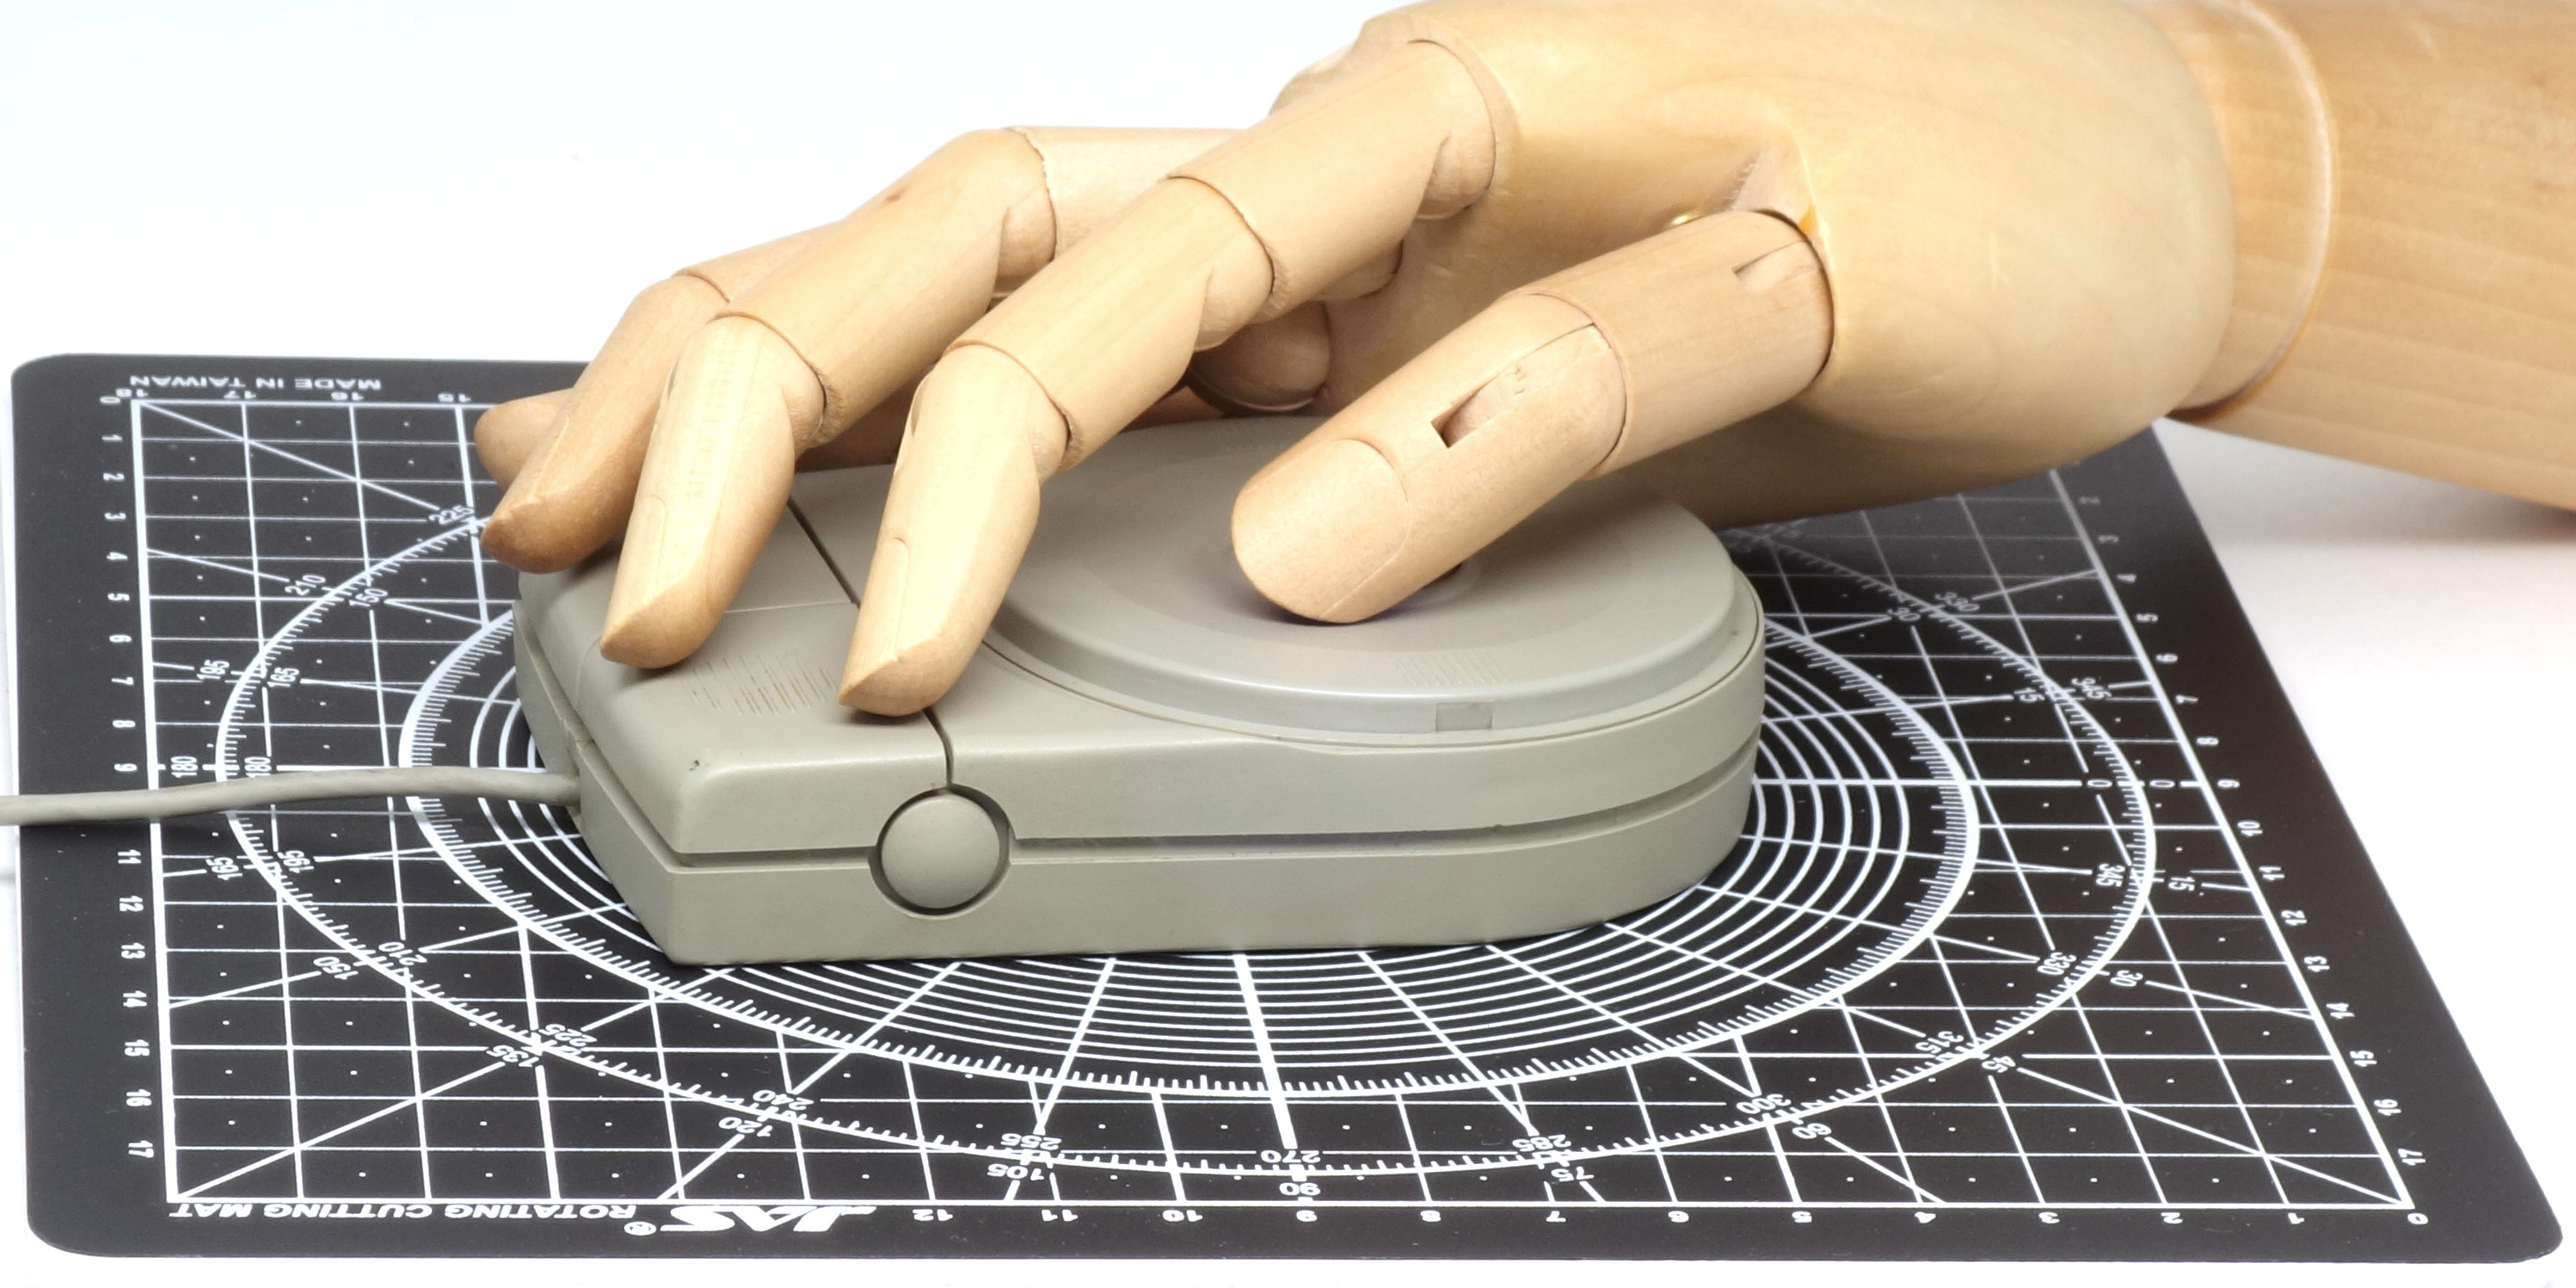
\includegraphics[scale=0.45]{1987_sharp_convertible/handball_30.jpg}
    \caption{Sharp KI-OM0002CE01 в режиме трекбола с моделью руки человека}
    \label{fig:SharpConvertibleBallHand}
\end{figure}

\begin{figure}[h]
    \centering
    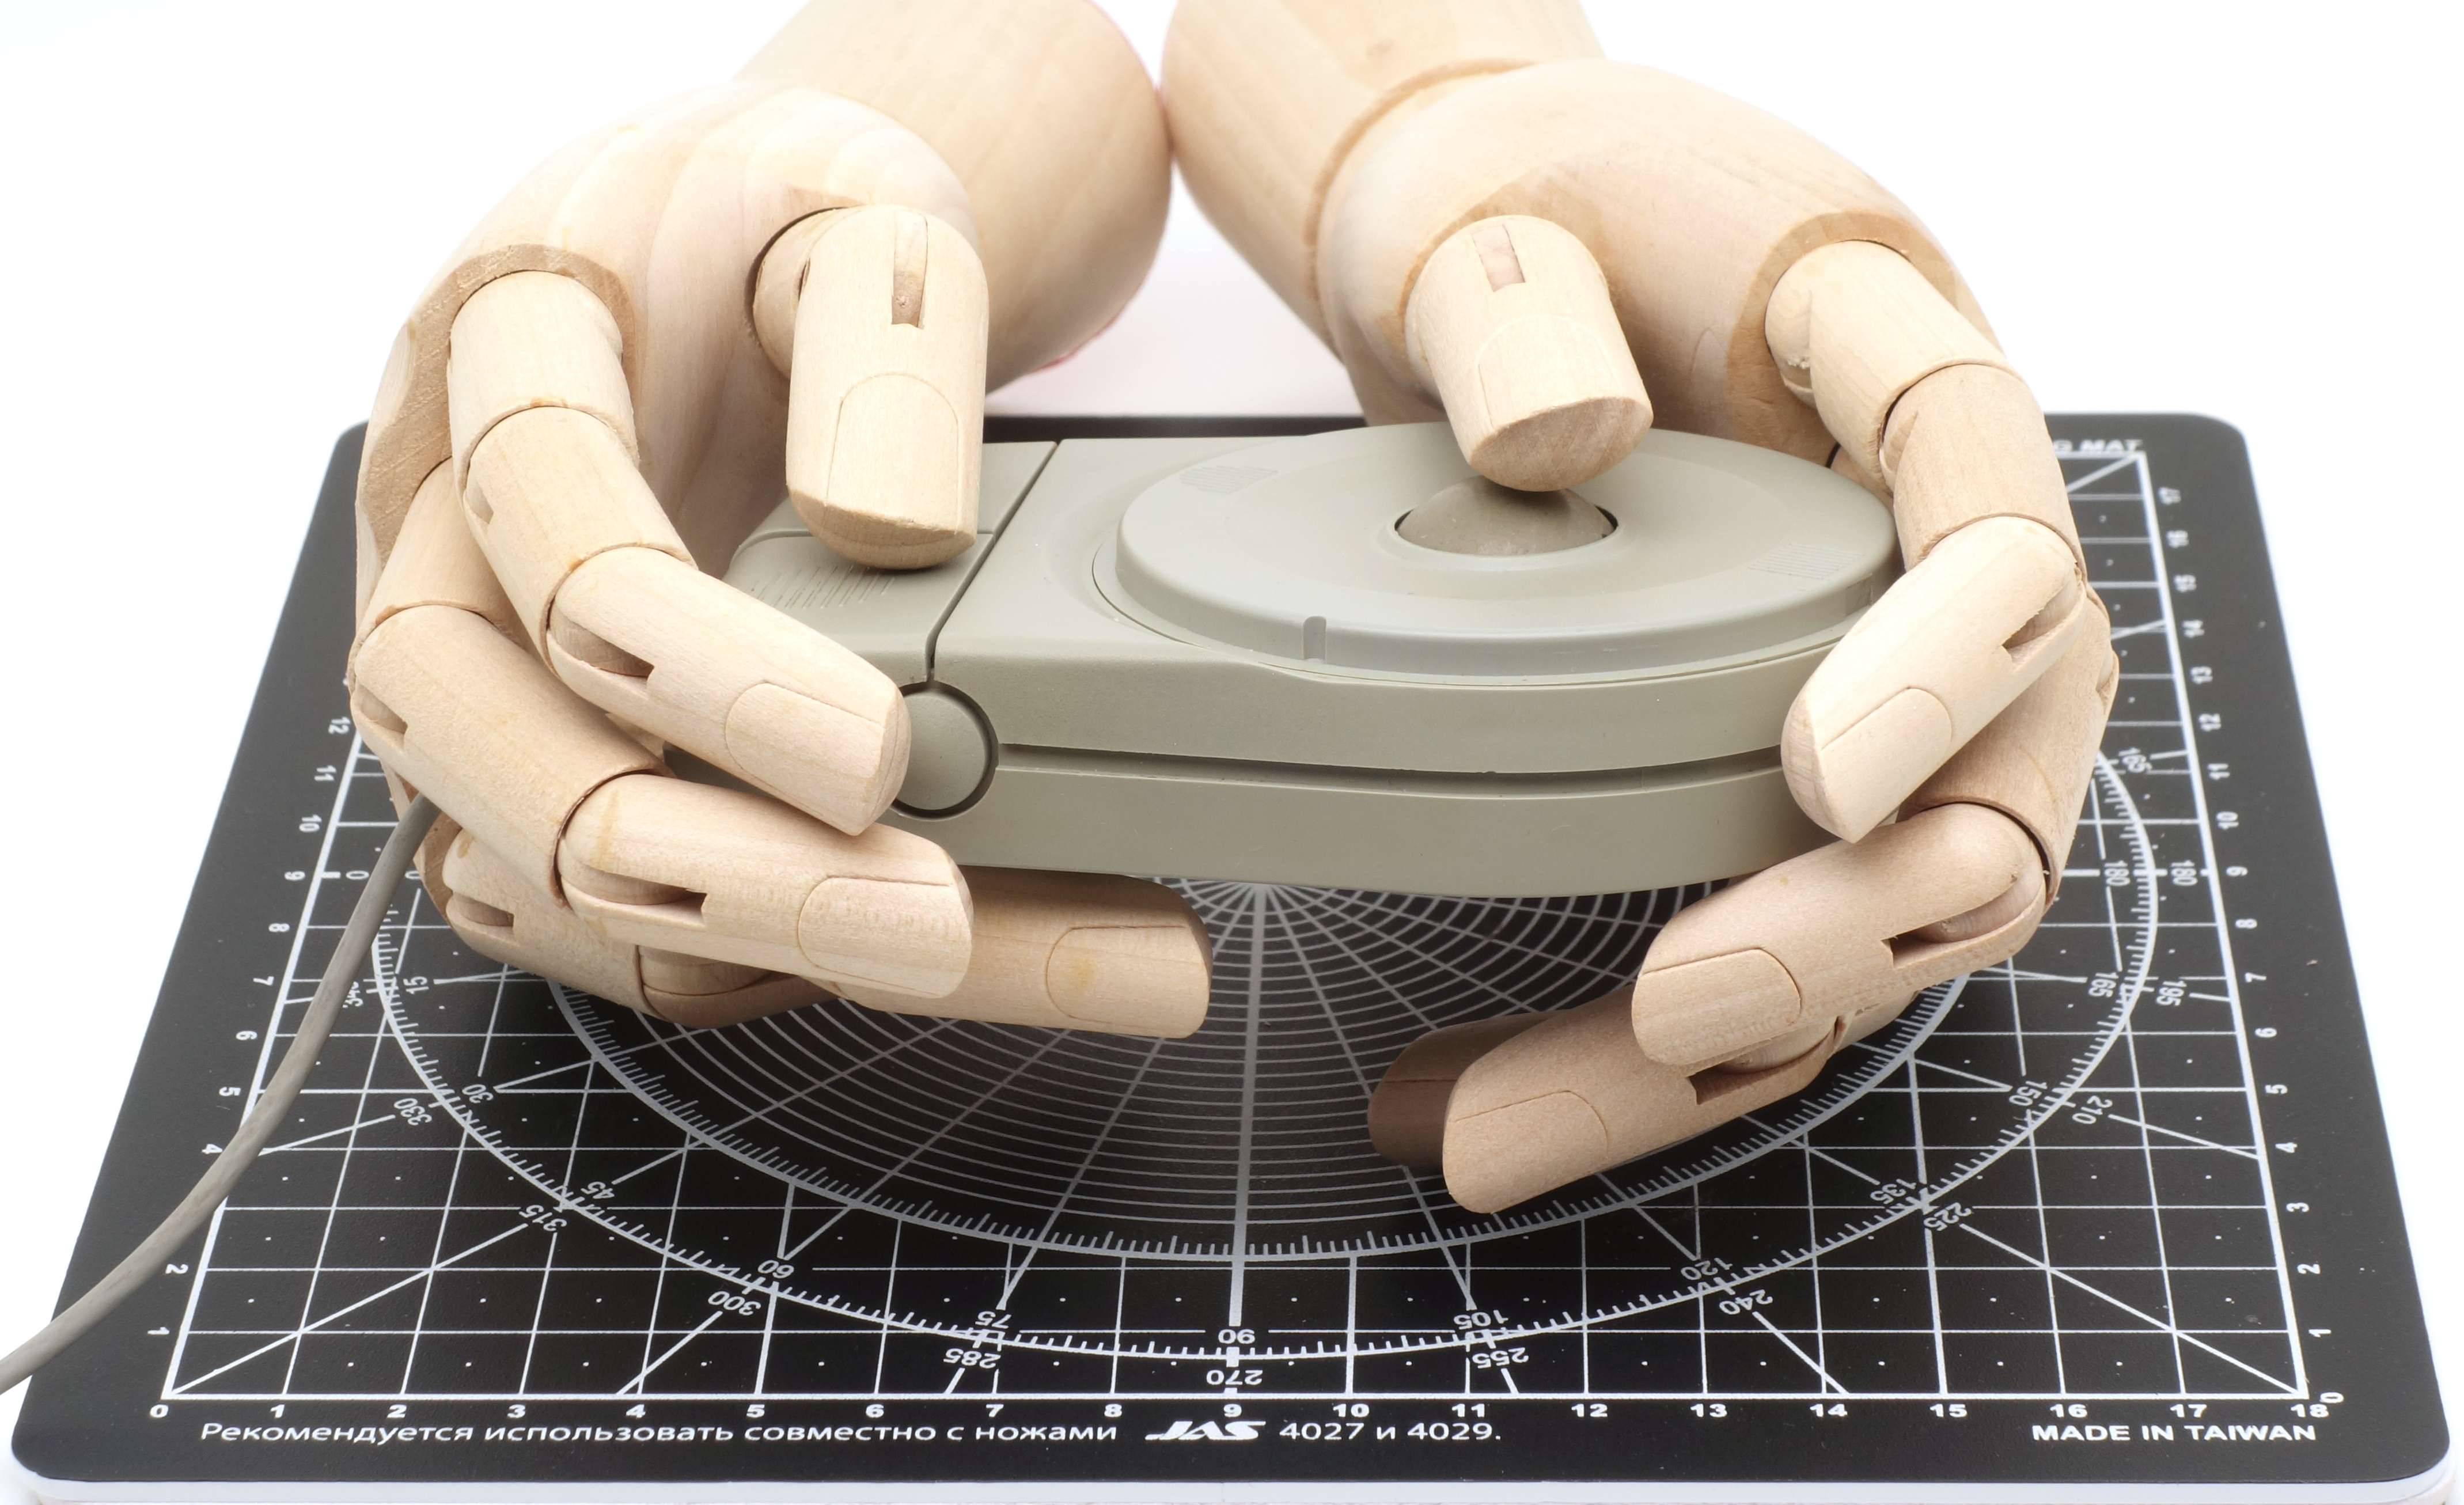
\includegraphics[scale=0.31]{1987_sharp_convertible/handpad_30.jpg}
    \caption{Sharp KI-OM0002CE01 в режиме геймпада}
    \label{fig:SharpConvertiblePadHand}
\end{figure}

Изучение разобранного трекбола показывает, что в нем использованы закрытые механические энкодеры, соответствующие ранним устройствам Alps, и характерные для них же металлические ролики с подшипниками качения. Помимо поворотного блока, мдификацией стандартной конструкции Alps является  отсутствие (из-за необходимости работы в режиме трекбола) глухой пластиковой защиты шара, типичной для мышей 80-х годов и упраздненной в более поздних моделях (рис. \ref{fig:SharpConvertibleInside}). Также следует отметить воронкообразную форму отверстия в корпусе, защищающую провод от повреждения (в последствии в компьютерных мышах для этой цели использовали ребристую защитную муфту).

\begin{figure}[h]
    \centering
    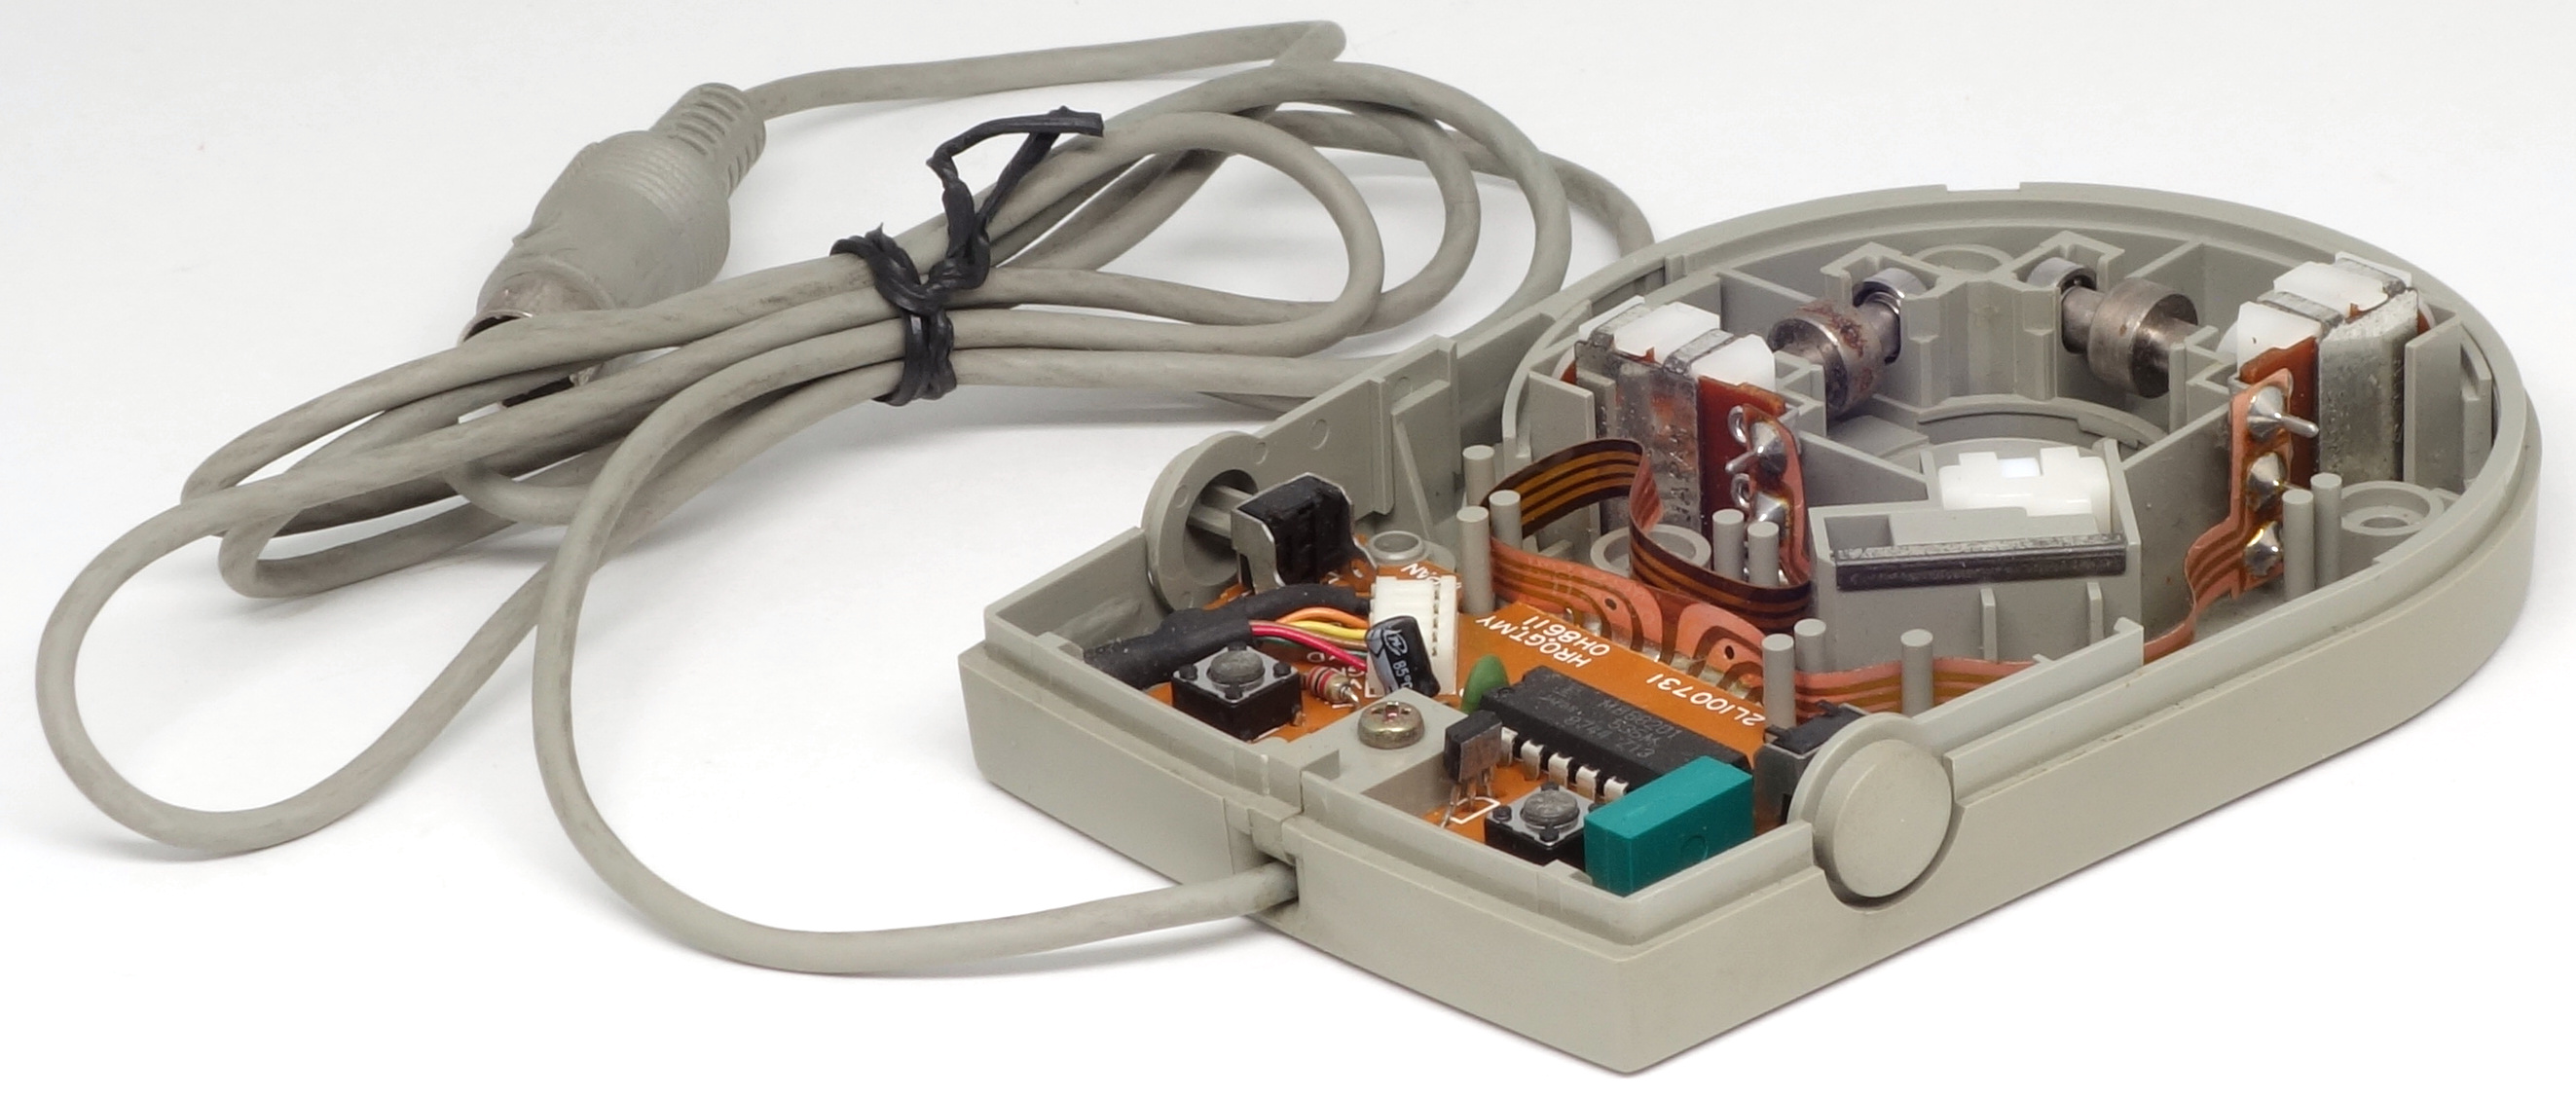
\includegraphics[scale=0.8]{1987_sharp_convertible/inside_30.jpg}
    \caption{Изображение KI-OM0002CE01 изнутри}
    \label{fig:SharpConvertibleInside}
\end{figure}

\begin{thebibliography}{9}
\bibitem {museum} X680000-Computer Museum \url{https://museum.ipsj.or.jp/en/computer/personal/0038.html}
\bibitem{JapaneseVintage} Sharp X86000 Expert -- Japanese Vintage Computer Collection. FEB 2, 2020 \url{https://monochromeeffect.org/JVCC/2020/02/02/x68000-expert/}
\bibitem{JapaneseClickSense} Otonashi. X68000 Z review [in Japanese] - GAME Watch, May 29, 2023 \url{https://game.watch.impress.co.jp/docs/review/rev1/1501505.html}
\end{thebibliography}
\end{document}
